\documentclass[12pt]{beamer}
\usetheme{Boadilla}

\usepackage[utf8]{inputenc}
\usepackage{graphicx}
\usepackage{amsmath}
\usepackage{tikz}

\setbeamersize{text margin left=10mm,text margin right=10mm}

\title{Simulation Methods for Finance}
\subtitle{Barrier and Look-back Options}
\author{Espel, Kulak, Qiu, Zhang}
\institute{Imperial College London}
\date{\today}

\begin{document}

\begin{frame}
    \titlepage
\end{frame}


\begin{frame}
\frametitle{Introduction}
\begin{itemize}
  \item Create a module for the core task: random variable generation, European option.
  \item Barrier option: price and greeks.
  \item Look-back option: price and greeks.
  \item Document the code and create a user manual.
\end{itemize}
\end{frame}



\begin{frame}
\frametitle{Outline}
\tableofcontents
\end{frame}


\section{Random Variable Generation}
\begin{frame}
\frametitle{Random Variable Generation - Task}

\end{frame}

\begin{frame}
\frametitle{Random Variable Generation - Analysis}

\end{frame}

\begin{frame}
\frametitle{Random Variable Generation - Results}

\end{frame}



\section{European Call Option}
\begin{frame}
\frametitle{European Call Option - Task}

With the usual conventions, recall our model.
$$dS_t=rS_tdt+\sigma S_tdW_t, \ 0\leq t \leq T$$
$$C_t = E[e^{-r(T-t)}(S_T-K)^+|\textit{F}_t]$$

\begin{itemize}
  \item Create a module to simulate the results for the European option.
  \item Compute the Greeks (delta, gamma, vega) using different methods.
  \item Analyse the error compared to the theoretical result.
\end{itemize}
\end{frame}

\begin{frame}
\frametitle{European Call Option - Analysis}
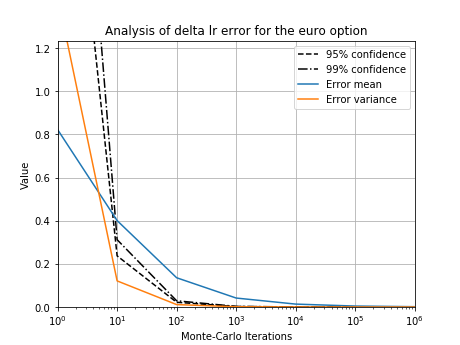
\includegraphics[width=.5\textwidth]{graphs/eurodeltalr.png}
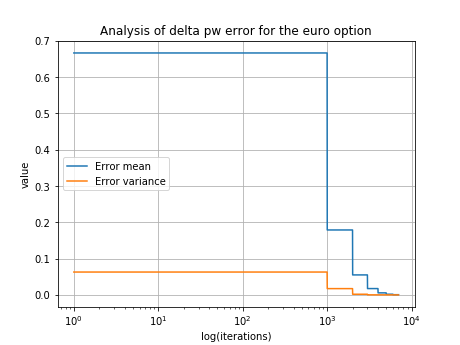
\includegraphics[width=.5\textwidth]{graphs/eurodeltapw.png}
\end{frame}

\begin{frame}
\frametitle{European Call Option - Analysis}
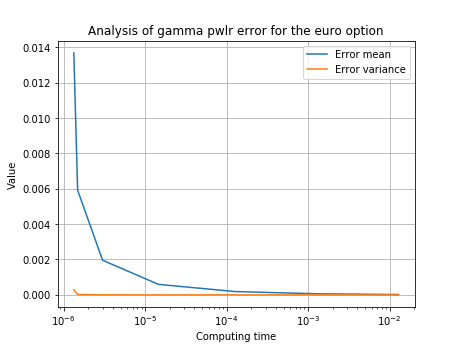
\includegraphics[width=.5\textwidth]{graphs/eurogammapwlrtime.png}
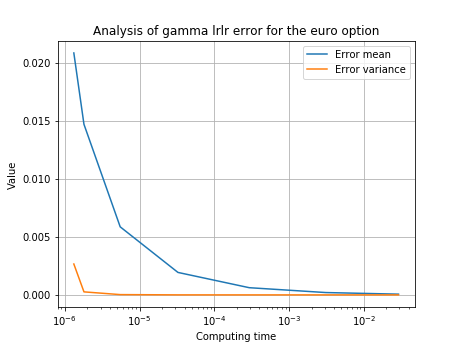
\includegraphics[width=.5\textwidth]{graphs/eurogammalrlrtime.png}
\end{frame}

\begin{frame}
\frametitle{European Call Option - Results}
\begin{itemize}
  \item There is a significant accuracy gap beyond 1,000 simulations.
  \item We based our conclusions on the industry standard: 100,000 simulations.
  \item There is a trade-off computation time/accuracy.
\end{itemize}



\begin{table}
  \centering
\begin{tabular}{|l|c|c|c|}
\hline
& \textbf{Error Mean} & \textbf{Error Variance} & \textbf{Time} \\ \hline
\textbf{Delta LR} & Worst & Worst & Best\\
\textbf{Delta PW} & Best & Best & Worst\\ \hline
\textbf{Gamma PWLR} & Worst & Best & Best\\
\textbf{Gamma LRPW} & - & Worst & Best\\
\textbf{Gamma LRLR} & - & - & Worst\\ \hline
\textbf{Vega LR} & Worst & - & Worst\\
\textbf{Vega PW} & Best & - & Best\\ \hline
\end{tabular}\\

\end{table}

\end{frame}




\section{Barrier Option}
\begin{frame}
\frametitle{Barrier Option - Task}

\end{frame}

\begin{frame}
\frametitle{Barrier Option - Analysis}
%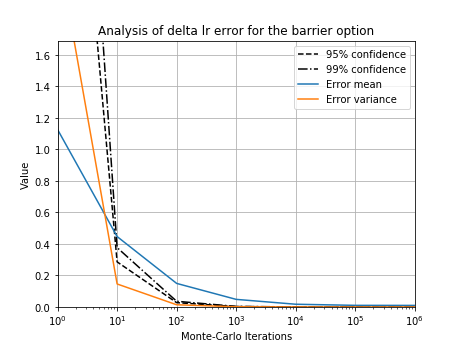
\includegraphics[width=.5\textwidth]{graphs/barrierdeltalr.png}
%\includegraphics[width=.5\textwidth]{graphs/barriergammalr.png}
\end{frame}

\begin{frame}
\frametitle{Barrier Option - Analysis with a New Method}
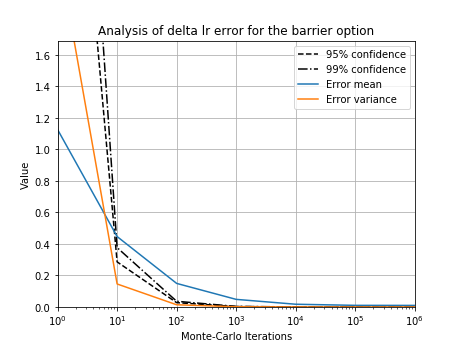
\includegraphics[width=.5\textwidth]{graphs/barrierdeltalr.png}
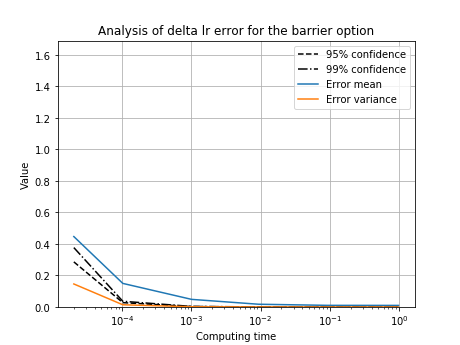
\includegraphics[width=.5\textwidth]{graphs/barrierdeltalrtime.png}
\end{frame}

\begin{frame}
\frametitle{Barrier Option - Analysis with a New Method}
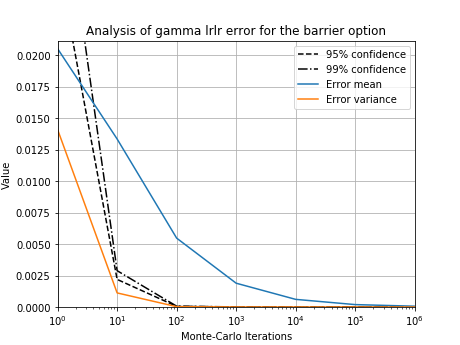
\includegraphics[width=.5\textwidth]{graphs/barriergammalrlr.png}
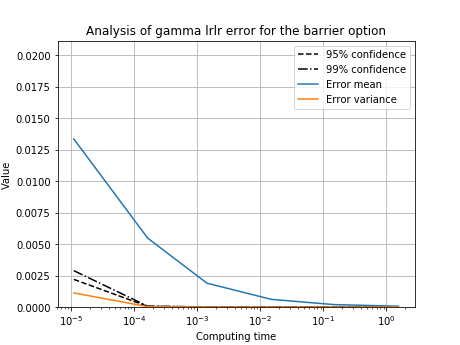
\includegraphics[width=.5\textwidth]{graphs/barriergammalrlrtime.png}
\end{frame}

\begin{frame}
\frametitle{Barrier Option - Results}

\end{frame}


\section{Look-back Option}
\begin{frame}
\frametitle{Look-back Option - Task}

\end{frame}

\begin{frame}
\frametitle{Look-back Option - Analysis}
%\includegraphics[width=.5\textwidth]{graphs/lookbdeltalr.png}
%\includegraphics[width=.5\textwidth]{graphs/lookbgammalr.png}
\end{frame}

\begin{frame}
\frametitle{Look-back Option - Results}

\end{frame}


\section{Using our Code}
\begin{frame}
\frametitle{Using our Code - C++ Package}
\begin{itemize}
  \item We have created a package for C++ users.
  \item Uses industry standards with dynamic library files.
  \item Package is very intuitive.
\end{itemize}

\begin{figure}[h!]
  \centering
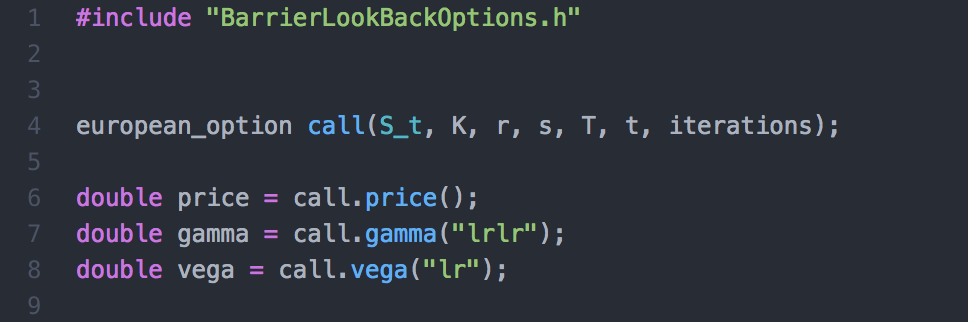
\includegraphics[width=\textwidth]{graphs/code_easy_demo.png}
\end{figure}
\end{frame}


\begin{frame}
\frametitle{Using our Code - "Code Free" terminal}
\begin{itemize}
  \item We have created an intuitive interface.
  \item This is suitable for users who do not code: you just have to type the command and there is a help mode.
  \item It supports european call option, barrier option and the look-back option price and delta.
\end{itemize}
\begin{figure}[h!]
  \centering
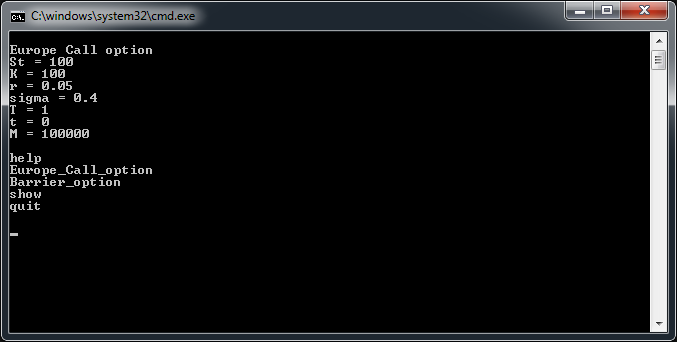
\includegraphics[width=.8\textwidth]{graphs/interface_demo.png}
\end{figure}
\end{frame}



\begin{frame}
\frametitle{Conclusion}
\begin{itemize}
  \item We have created a module with the core task.
  \item The module also can also compute elements related to the barrier option and the look-back option.
  \item Our package is user-friendly and has a "code-free" interface.
\end{itemize}
\end{frame}



\begin{frame}

\centering
{\Large Thank you!}
\\[1cm]
{\small\url{github.com/tjespel/barrier-and-look-back-options}}
\end{frame}

\end{document}
